\documentclass[../../main.tex]{subfiles}

\subsubsection{Erste Ideen}

Im folgenden Beitrag werde Ich meine Ideen und Optionen zum Thema „Spiele – Digital“ mit Berücksichtigung auf technische Einschränkungen und andere Faktoren aufführen.

Vorweg liste ich die theoretisch möglichen Optionen auf. Diese sind aufzugliedern in Hardware und Software. Im Bereich der Hardware ist für die Maschine, auf der die Spiele laufen, ist sowohl ein PC, als auch eine Konsole (Xbox, Switch, etc.) machbar. Außerdem stellt sich die Frage, welche Eingabemethode angeboten werden soll. Hierfür bieten sich u. A. Controller oder Tastatur mit Maus an. Bei der Aufgabe der Spiele ist so gut wie alles machbar. Anbieter hierfür wären bei Konsolen deren Hersteller (Microsoft, Nintendo, etc.) und bei PCs eine Reihe an Spielehändlern wie Steam, Epic Games, etc.

Welche Option ist also die Richtige? Um diese Frage zu beantworten, müssen einige Faktoren beachtet werden. Zur Entscheidungsfindung sind Statistiken v. a. im Bereich Spielesortiment besonders wichtig. Mithilfe der Informationen in Hinsicht auf Spieleranzahl und Bewertungen kann man sich auf eine bessere Auswahl einschränken. Zusätzlich sind Umfragen für außergewöhnlichere Themen und Fragen Bezüglich der Hardware besonders wichtig. Diese können mit Klinikspezifischen Fragen erstellt werden, und sind somit die Ausschlaggebendste Quelle.

Des Weiteren gibt es Dinge, die bei Klinikpatienten zu berücksichtigen sind. Zum einen befasse ich mich mit dem Thema der Inklusion und Barrierefreiheit. Um körperlich eingeschränkte Menschen einzubinden, müssen Eingabemethoden angepasst werden (z. B. Sprachsteuerung). Zugleich muss das Problem der Einsamkeit des Patienten angegangen werden. Ein möglicher Lösungsansatz wären Online-Spiele, die mit Freunden gespielt werden können. Überdies wird das Spieleangebot von kurz untergebrachten Patienten selten angenommen, da sie sich in einer stressigen Situation befinden. Sogenannte „Hyper Casual Games“ sind ein Mittel, um diesen Personen Stress abzunehmen.

Kommen wir nun zu meinen persönlichen themenbezogenen Ideen. In Bezug auf Interoperabilität mit anderen Aufgaben der Gestaltung der Klinik gibt es die Möglichkeit, die Hardware zu teilen. Das Thema „Spiele – Digital“ für die Altersgruppe 6-11 wird mit Sicherheit viele Ähnlichkeiten mit meinem haben. Das gleiche gilt für das Thema „Unterhaltung“ – hier bieten sich sowohl PC als auch Xbox als Mediengeräte an.

Im Hinblick auf die Hardware bietet sich an, die Ausstattung zu erweitern. Pro zwei-Betten-Zimmer befindet sich ein Fernseher, den sich beide Patienten teilen müssen. Einen weiteren zu installieren ist ein Weg, die Erfahrung zu verbessern. Des Weiteren könnte man ein Konsolen-Ausleihsystem mit umfassender Auswahl einführen, um den Anforderungen jedes Besuchers gerecht zu werden. 

Zum Thema Software gibt es die Gelegenheit, eine spezielle Benutzeroberfläche zu erstellen, welche mit dem Angebot der Unterhaltung vereinbar ist. Somit können Nutzer problemlos im System navigieren.

Schlussendlich kommen wir zum Fazit. Es gibt eine Reihe an realistischen Optionen, Besuchern Digitale Spiele als Freizeitaktivität zu bieten. Man kann ein vielseitiges System anfertigen, das in Einklang mit anderen Aufgaben der Gestaltung der Klinik steht. Trotzdem muss man bei der finalen Entscheidung immer auf Umfragen und Einschränkungen achten.

\subsubsection{Konkrete architektorische Ideen}

Im Folgenden Text betrachten wir meine Konzepte bezüglich Videospielen in einer Kinderklinik und deren Übertrag in die Architektur. Da die Umfrageauswertung ausschlaggebende Informationen zu den Bedürfnissen potentieller Patienten gibt, stelle ich meine Ideen auch im Bezug dieser dar. Im Gegensatz zum Thema der Gerätegestaltung gibt es hier keine große Gefahr, Kinder mit einem unangenehmen Design abzuschrecken; trotzdem ist es wichtig, den Patientenaufenthalt auch durch die visuelle Gestaltung der Spielegeräte im Rahmen meiner Möglichkeiten angenehm zu machen.

So habe ich z. B. ein Konsolendesign konzipiert, welches zum Raumdesign der Klinik passt und nicht zu sehr heraussticht (Abb. \ref{fig:konsolendesign}).

Gegen den Einsatz eines solchen Designs spricht jedoch, dass es mit Sicherheit dem Patienten Fremd sein würde und kein Gefühl von Familiarität erwecken würde.

Ein wichtigerer und weniger ambiguöser Teil ist das Verstecken von Kabeln. In einem Patientenzimmer gibt es oft schon genügend gruselige Maschinen und Kabel - das muss beim Gaming-System nicht sein. Gutes Kabel-Management ist also gerade hier notwendig für ein positives visuelles Bild der Geräte. Führen wir alle Kabel zwischen Fernseher und Konsole zusammen, ist das Problem schon gelöst (Abb. \ref{fig:cable_management}). Darüber hinaus verwenden wir natürlich drahtlose Controller - eine Substantielle Verzögerung ist nicht Vorhanden.


Da die förderung von selbstgebrachten Konsolen laut Umfrageergebnissen durchaus erwünscht ist, musste ich mir auch hierzu etwas einfallen lassen. Weil die Nintendo Switch, Smartphones und Laptops zu den bedeutendsten tragbaren Konsolen gehören, maßschneidere ich meine Ideen vor Allem auf diese. Für alle drei wäre es grundlegend wichtig, sowohl eine Möglichkeit zum Aufladen, als auch kostenloses WLAN für Patienten und Besucher anzubieten. Man könnte auch spezifisch für die Nintendo Switch ein Dock installieren, das bereits an den Fernseher angeschlossen ist.

% BILD DOCK

Das Software-UI wird größtenteils durch die Hardware bestimmt: Die Schaltoberfläche kommt mit der Konsole. Verwenden wir aber einen PC, was laut Umfrage nicht unattraktiv ist, sind die möglichkeiten grenzenlos. Am einfachsten wäre hier Steam Big Picture Mode (Abb. \ref{fig:big_picture}) - eine Schaltfläche, welche der von Konsolen ähnelt, also auch Controllergesteuert. Es bietet sich aber auch an, ein eigenes UI zu entwickeln, das möglicherweise auch Multimedia-Entertainment mit Videospielen vereint.

Am wichtigsten ist in meinen Augen aber, ein Gefühl von Normalität zu vermitteln. Daher sollten Ideen wie ein eigenes Konsolendesign möglicherweise nicht umgesetzt werden. Wichtig ist trotzdem wie gesagt das Angebot von WLAN und Strom.

\begin{figure}[h!]
    \centering
    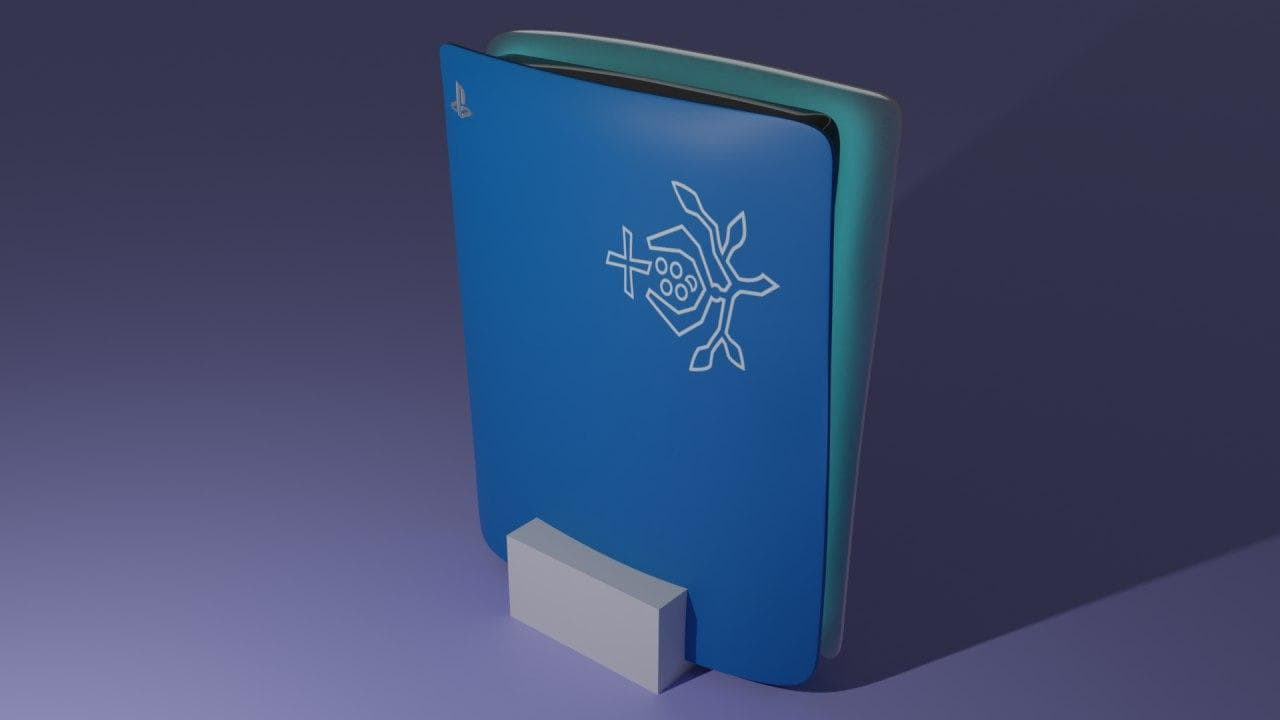
\includegraphics[width=\textwidth]{ps5_branded.jpg}
    \caption{PS5 mit Logo der Barmherzigen Brüder. \footnotesize{(``Sony PlayStation 5'' by Spellmansp is licensed under Creative Commons Attribution. https://skfb.ly/6UtSN To view a copy of this license, visit http://creativecommons.org/licenses/by/4.0/.)}}
    \label{fig:konsolendesign}
\end{figure}

\begin{figure}[h!]
    \centering
    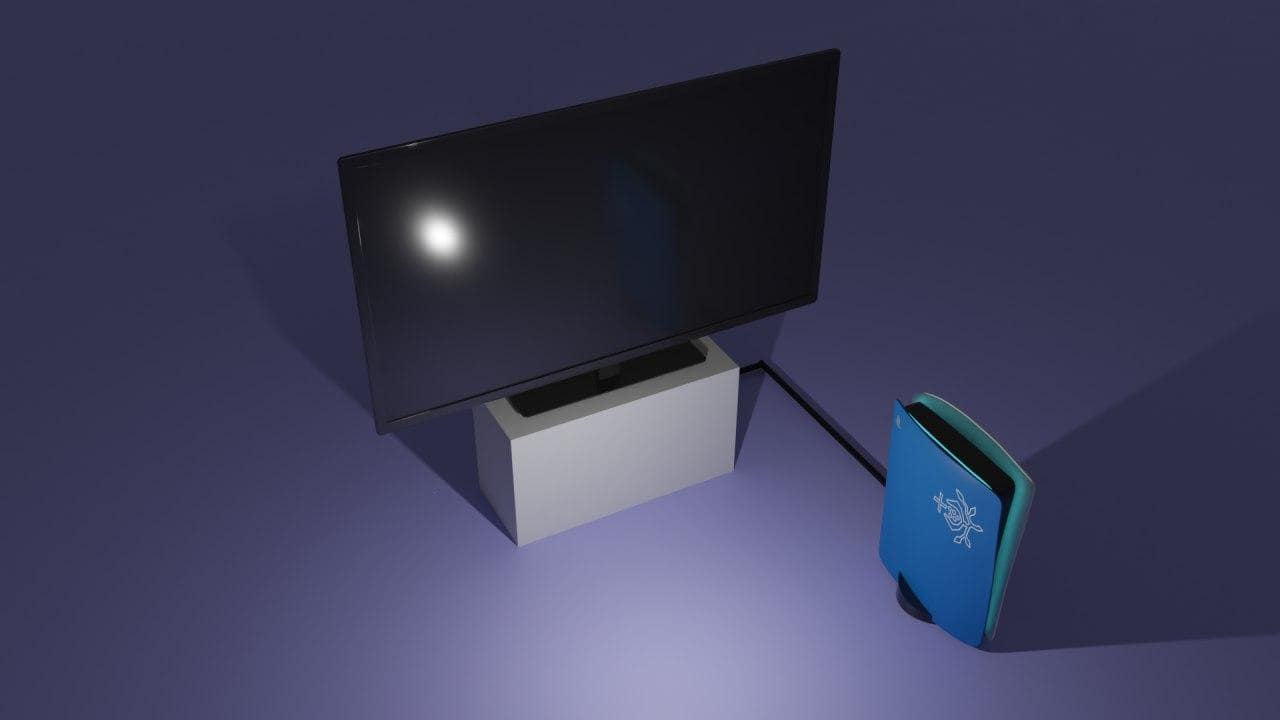
\includegraphics[width=\textwidth]{ps5_cablemanagement.jpg}
    \caption{Kabelmanagement. \footnotesize{("Flatscreen TV 46 inch" by thethieme is licensed under Creative Commons Attribution. https://skfb.ly/DBrF To view a copy of this license, visit http://creativecommons.org/licenses/by/4.0/.)}}
    \label{fig:cable_management}
\end{figure}

\begin{figure}[h!]
    \centering
    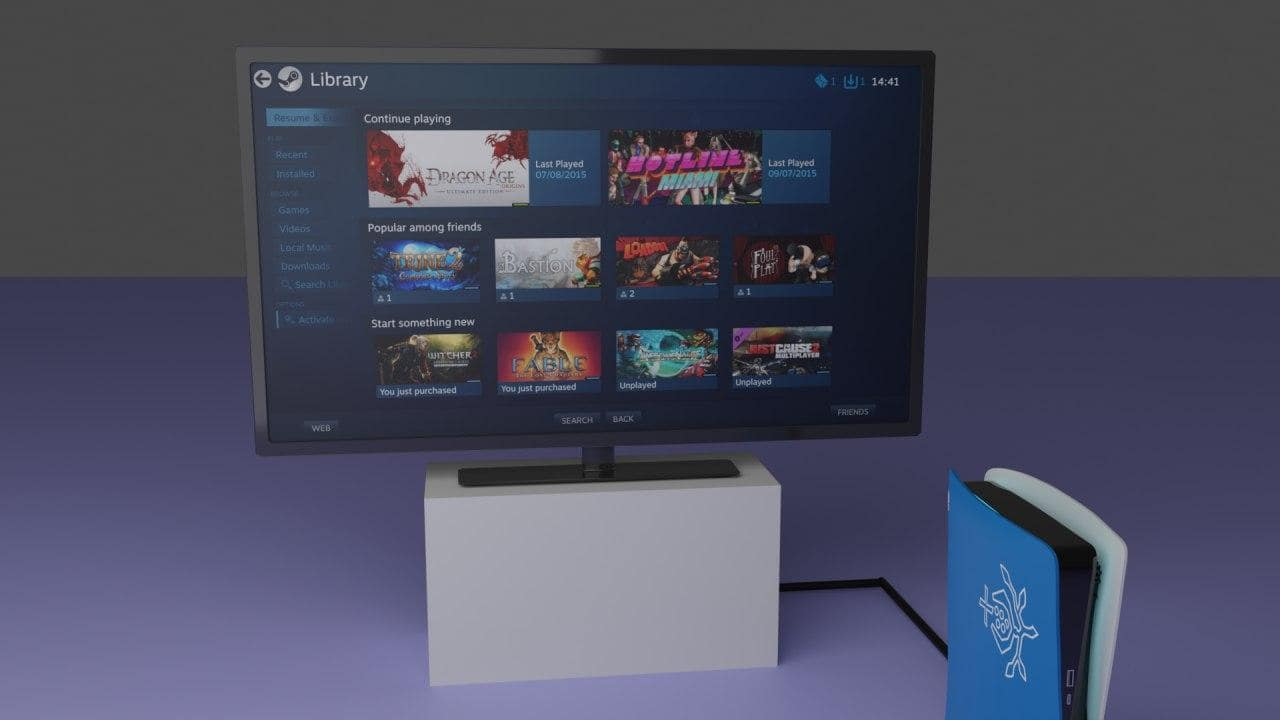
\includegraphics[width=\textwidth]{ps5_steam.jpg}
    \caption{Steam Big Picture}
    \label{fig:big_picture}
\end{figure}
